\subsection{Curva de calibración}

Los datos obtenidos de densidad óptica desde una muestra con número de células viables de detalla en la tabla \ref{tab:cal_brut}

\begin{table}[H]
  \centering
  \begin{tabular}{ccccccccc}\toprule
    & \multicolumn{7}{c}{Dilución en relación a muestra original} & \\ \cmidrule{2-8}
    & 1:2 & 1:4 & 1:8 & 1:16 & 1:32 & 1:64 & 1:128 & Blanco \\ \cmidrule{2-9}
    & 0.905 & 0.537 & 0.307 & 0.183 & 0.110 & 0.077 & 0.061 & 0.044 \\
    & 0.905 & 0.537 & 0.303 & 0.178 & 0.111 & 0.077 & 0.059 & 0.042 \\
    & 0.918 & 0.542 & 0.310 & 0.180 & 0.113 & 0.077 & 0.061 & 0.041 \\ \midrule
    Promedio & 0.909 & 0.539 & 0.307 & 0.180 & 0.111 & 0.077 & 0.060 & 0.042 \\ \bottomrule
  \end{tabular}
  \caption{Densidad óptica muestras con \si{\ufc\per\mL} conocida (datos en bruto)}
  \label{tab:cal_brut}
\end{table}


Se ajustaron los datos para obtener la densidad óptica de la muestra, ya que la presentada en la tabla \ref{tab:cal_brut} indica la densidad óptica tanto del organismo como del medio de cultivo, lo que son presentado en la tabla \ref{tab:cal_adj}

\begin{table}[H]
  \centering
  \begin{tabular}{cccccccc}\toprule
    & \multicolumn{7}{c}{Dilución en relación a muestra original} \\ \cmidrule{2-8}
    & 1:2 & 1:4 & 1:8 & 1:16 & 1:32 & 1:64 & 1:128 \\ \cmidrule{2-8}
    & 0.861 & 0.493 & 0.263 & 0.139 & 0.066 & 0.033 & 0.017 \\
    & 0.863 & 0.495 & 0.261 & 0.136 & 0.069 & 0.035 & 0.017 \\
    & 0.877 & 0.501 & 0.269 & 0.139 & 0.072 & 0.036 & 0.02 \\ \midrule
    Promedio & 0.867 & 0.496 & 0.264 & 0.138 & 0.069 & 0.035 & 0.018 \\ \bottomrule
  \end{tabular}
  \caption{Densidad óptica muestras con \si{\ufc\per\mL} conocida (datos corregidos)}
  \label{tab:cal_adj}
\end{table}

Dado que el inocuo inicial contenía \SI{4.5e9}{\ufc\per\mL}, los títulos de las diluciones seriadas están totalmente determinado y se adjuntan en la siguiente tabla

\begin{table}[H]
  \centering
  \begin{tabular}{cc}\toprule
    Dilución & Título ($\times$\SI{e9}{\ufc\per\mL}) \\ \midrule
    1:2 & 2.25 \\
    1:4 & 1.12 \\
    1:8 & 0.562 \\
    1:16 & 0.281 \\
    1:32 & 0.141 \\
    1:64 & 0.0704 \\
    1:128 & 0.0352 \\ \bottomrule
  \end{tabular}
  \caption{Título diluciones}
  \label{tab:tab_title}
\end{table}

Entonces, a partir de los datos experimentales detallados previamente, es que se construyó una \emph{curva de calibración} que relaciona la densidad óptica (DO) medida con la cantidad de células viables (\si{\ufc\per\mL}), la que ilustra en la figura \ref{fig:cal_curve}

\begin{figure}[H]
  \centering
  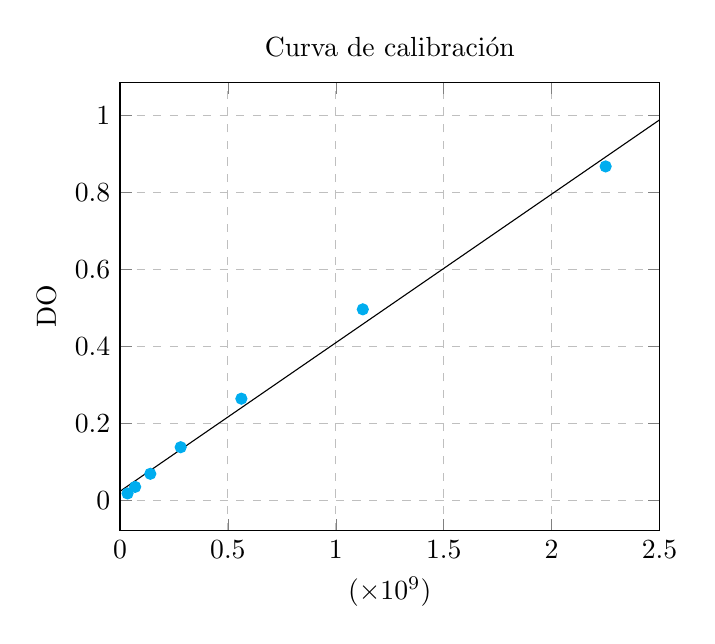
\begin{tikzpicture}[baseline=(current bounding box.center)]
    \begin{axis}[
        title={Curva de calibración}, 
        xlabel={\si{\ufc\per\mL}($\times10^9$)},
        ylabel={DO},
        xmin=0, xmax=2.5,
        xticklabel style={ 
          /pgf/number format/precision=3, 
          /pgf/number format/fixed}, 
        legend pos = north west, 
        ymajorgrids=true, 
        xmajorgrids=true, 
        yminorgrids=true, 
        xminorgrids=true, 
        grid style=dashed]

      \addplot[only marks, color=cyan]
        coordinates {
          (2.25, 0.867)
          (1.125, 0.496)
          (0.5625, 0.264)
          (0.28125, 0.138)
          (0.140625, 0.069)
          (0.0703125, 0.035)
          (0.03515625, 0.018)
        };

      \addplot[no marks] {0.385792*x+0.0235};

    \end{axis}
  \end{tikzpicture}
  \caption{Curva de calibración}
  \label{fig:cal_curve}
\end{figure}

De los datos presentados en la tabla \ref{tab:cal_adj} y la figura \ref{fig:cal_curve}, y según el método de mínimos cuadrados, la recta de mejor ajuste se determinó y corresponde a 

\begin{equation}
  \text{DO}(n)=0.385792\cdot n + 0.0235
  \label{eq:first_model}
\end{equation}

donde $n$ corresponde a la mantisa del valor de las células viables cuando éstas están expresadas en orden de magnitud 9, e.g., si el número de células viables es de \SI{2.25e9}{\ufc\per\mL} entonces el valor que ingresa a la función es 2.25, teniendo este modelo un coeficiente de determinación $R^2=0.994256$.

Se manipuló el modelo presentado en la ecuación \eqref{eq:first_model} de forma algebraica para obtener un segundo modelo, 

\begin{equation}
  n(\text{DO}) = 2.57718\cdot \text{DO}-0.0569
  \label{eq:actual_model}
\end{equation}

, donde $\text{DO}$ representa la densidad óptica medida y $n$, tal como se indicó más arriba, la mantisa del número de células viables cuando el orden de magnitud es 9.

\subsection{Curva de crecimiento}

Las mediciones de densidad óptica obtenidas para muestra problema se detallan en la tabla \ref{tab:growth_brut}. 

Los datos presentado en la tabla \ref{tab:growth_brut} se corrigieron, en su promedio, los cuales se presentan en la tabla \ref{tab:growth_fixed}.

\begin{table}[H]
  \centering
  \begin{tabular}{cccc}\toprule
    & Glicerol & Sucrosa & Glucosa \\ \cmidrule{2-4}
    \multirow{3}{*}{$t=\SI{0}{\minute}$} & 0.066 & 0.067 & 0.072 \\
    & 0.067 & 0.069 & 0.069 \\
    & 0.064 & 0.070 & 0.070 \\ 
    Promedio & 0.066 & 0.069 & 0.070 \\ \midrule
    \multirow{3}{*}{$t=\SI{30}{\minute}$} & 0.084 & 0.102 & 0.111 \\
    & 0.091 & 0.102 & 0.105 \\
    & 0.082 & 0.111 & 0.119 \\
    Promedio & 0.086 & 0.105 & 0.112 \\ \midrule
    \multirow{3}{*}{$t=\SI{60}{\minute}$} & 0.111 & 0.139 & 0.153 \\
    & 0.116 & 0.143 & 0.145 \\
    & 0.105 & 0.139 & 0.153 \\
    Promedio & 0.111 & 0.140 & 0.150 \\ \midrule
    \multirow{3}{*}{$t=\SI{90}{\minute}$} & 0.160 & 0.162 & 0.241 \\
    & 0.163 & 0.165 & 0.241 \\
    & 0.156 & 0.174 & 0.240 \\
    Promedio & 0.160 & 0.167 & 0.241 \\ \midrule
    \multirow{3}{*}{$t=\SI{120}{\minute}$} & 0.233 & 0.186 & 0.342\\
    & 0.238 & 0.189 & 0.325 \\
    & 0.219 & 0.196 & 0.352 \\
    Promedio & 0.230 & 0.190 & 0.340 \\ \midrule
    Blanco & 0.037 \\ \bottomrule
  \end{tabular}
  \caption{Densidad óptica muestras con \si{\ufc\per\mL} desconocido (datos en bruto)}
  \label{tab:growth_brut}
\end{table}

\begin{table}[H]
  \centering
  \begin{tabular}{cccc}\toprule
    & Glicerol & Sucrosa & Glucosa \\ \cmidrule{2-4}
    $t=0$ & 0.029 & 0.032 & 0.033 \\ 
    $t=30$ & 0.049 & 0.067 & 0.075 \\ 
    $t=60$ & 0.074 & 0.103 & 0.113 \\ 
    $t=90$ & 0.123 & 0.130 & 0.204 \\ 
    $t=120$ & 0.193 & 0.153 & 0.303 \\ \bottomrule
  \end{tabular}
  \caption{Densidad óptica promedio muestras con \si{\ufc\per\mL} desconocido (datos corregidos)}
  \label{tab:growth_fixed}
\end{table}

Estos datos fueron graficados y dicho gráfico se muestra en la figura \ref{fig:growth_curve}.

Usando el modelo descrito en la ecuación \eqref{eq:actual_model} se interpolaron los datos presentado en la tabla \ref{tab:growth_fixed}; estos datos se tabularon y se encuentran disponbles en la tabla \ref{tab:growth_ufc}

\begin{figure}[H]
  \centering
  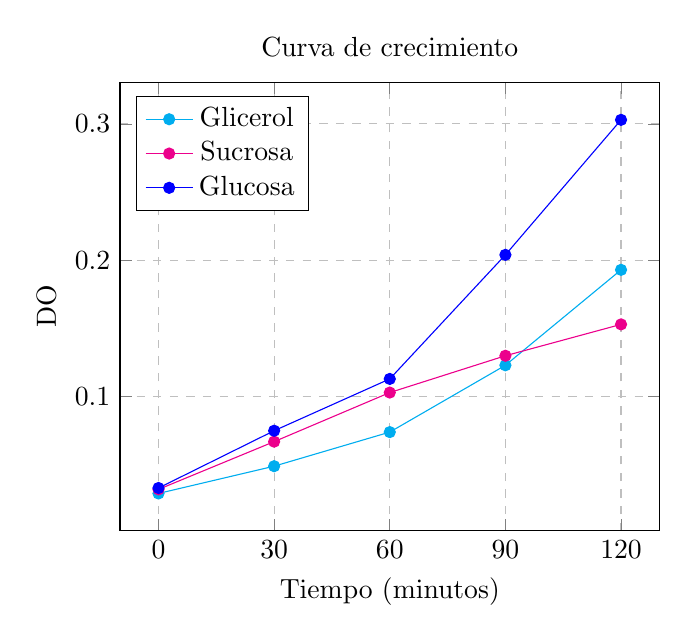
\begin{tikzpicture}[baseline=(current bounding box.center)]
    \begin{axis}[
        title={Curva de crecimiento}, 
        xlabel={Tiempo (minutos)},
        ylabel={DO},
        xmin=-10, xmax=130,
        xtick={0, 30, 60, 90, 120},
        xticklabel style={ 
          /pgf/number format/precision=3, 
          /pgf/number format/fixed}, 
        legend pos = north west, 
        yticklabel style={ 
          /pgf/number format/precision=3, 
          /pgf/number format/fixed}, 
        legend pos = north west, 
        ymajorgrids=true, 
        xmajorgrids=true, 
        yminorgrids=true, 
        xminorgrids=true, 
        grid style=dashed]

      \addplot[mark=*, color=cyan]
        coordinates {
          (0, 0.029)
          (30, 0.049)
          (60, 0.074)
          (90, 0.123)
          (120, 0.193)
        };
        \addlegendentry{Glicerol};

      \addplot[mark=*, color=magenta]
        coordinates {
          (0, 0.032)
          (30, 0.067)
          (60, 0.103)
          (90, 0.130)
          (120, 0.153)
        };
        \addlegendentry{Sucrosa};

      \addplot[mark=*, color=blue]
        coordinates {
          (0, 0.033)
          (30, 0.075)
          (60, 0.113)
          (90, 0.204)
          (120, 0.303)
        };
        \addlegendentry{Glucosa};

    \end{axis}
  \end{tikzpicture}
  \caption{Curva de crecimiento}
  \label{fig:growth_curve}
\end{figure}

\begin{table}[H]
  \centering
  \begin{tabular}{cccc}\toprule
    & Glicerol & Sucrosa & Glucosa \\ \cmidrule{2-4}
    $t=0$ & 0.01784 & 0.02557 & 0.02815 \\ 
    $t=30$ & 0.06938 & 0.1158 & 0.1364 \\ 
    $t=60$ & 0.1338 & 0.2085 & 0.2343 \\ 
    $t=90$ & 0.2601 & 0.2781 & 0.4688 \\ 
    $t=120$ & 0.4405 & 0.3374 & 0.7240 \\ \bottomrule
  \end{tabular}
  \caption{Interpolación de la DO para obtener \si{\ufc\per\mL}($\times10^9$)}
  \label{tab:growth_ufc}
\end{table}

Estos datos también fueron graficados, lo que se ilustra en la figura \ref{fig:growth_ufc}.

Se asume que este crecimiento es descrito mediante una progresión geométrica de la forma 

\begin{equation}
  N(t) = N_0 2^{n(t)}
  \label{eq:geom}
\end{equation}

en donde $n(t)$ es el número de generaciones transcurridas en un determinado tiempo $t$ (minutos para este caso), $N_0$ es la cantidad inicial de microorganismos y $N(t)$ es la cantidad de microorganismos como función del tiempo, siendo estas últimas expresadas en \si{\ufc\per\mL}.

Para efectos prácticos de cálculo, el modelo presentado en \eqref{eq:geom} se linealizó mediante el uso logaritmos naturales, tal como se expresa a continuación 

\begin{align}
  \Rightarrow\ln(N(t)) & = \ln\left(N_02^{n(t)}\right) \nonumber \\
  \Leftrightarrow \ln(N(t)) & =  n(t)\ln(2) + \ln(N_0)
  \label{eq:growth_line}
\end{align}

\begin{figure}[H]
  \centering
  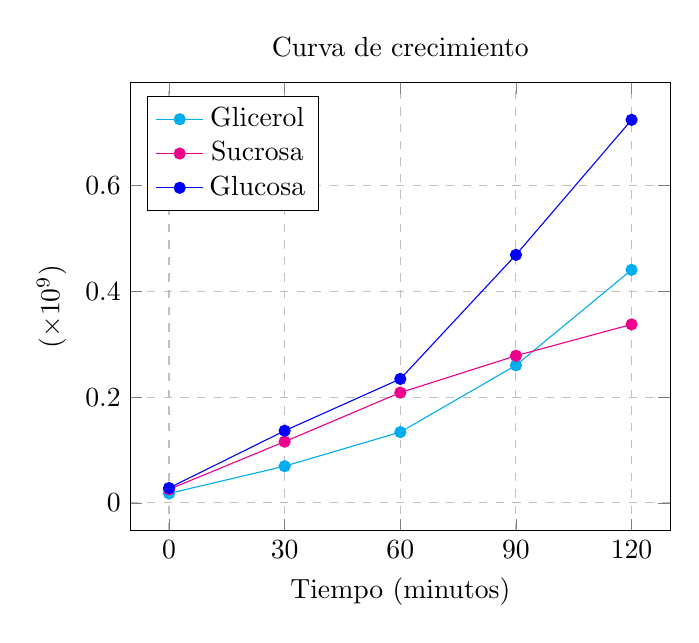
\begin{tikzpicture}[baseline=(current bounding box.center)]
    \begin{axis}[
        title={Curva de crecimiento}, 
        xlabel={Tiempo (minutos)},
        ylabel={\si{\ufc\per\mL}($\times 10^9$)},
        xmin=-10, xmax=130,
        xtick={0, 30, 60, 90, 120},
        xticklabel style={ 
          /pgf/number format/precision=3, 
          /pgf/number format/fixed}, 
        legend pos = north west, 
        yticklabel style={ 
          /pgf/number format/precision=3, 
          /pgf/number format/fixed}, 
        legend pos = north west, 
        ymajorgrids=true, 
        xmajorgrids=true, 
        yminorgrids=true, 
        xminorgrids=true, 
        grid style=dashed]

      \addplot[mark=*, color=cyan]
        coordinates {
          (0, 0.01784)
          (30, 0.06938)
          (60, 0.1338)
          (90, 0.2601)
          (120, 0.4405)
        };
        \addlegendentry{Glicerol};

      \addplot[mark=*, color=magenta]
        coordinates {
          (0, 0.02557)
          (30, 0.1158)
          (60, 0.2085)
          (90, 0.2781)
          (120, 0.3374)
        };
        \addlegendentry{Sucrosa};

      \addplot[mark=*, color=blue]
        coordinates {
          (0, 0.02815)
          (30, 0.1364)
          (60, 0.2343)
          (90, 0.4688)
          (120, 0.7240)
        };
        \addlegendentry{Glucosa};

    \end{axis}
  \end{tikzpicture}
  \caption{Curva de crecimiento}
  \label{fig:growth_ufc}
\end{figure}

El tiempo generacional, denotado por $g$, se define como

\begin{equation}
  g = \frac{t}{n}
  \label{eq:gen_time}
\end{equation}

Al calcular el recíproco del tiempo generacional es que se puede obtener la velocidad de crecimiento del microorganismo. 

Al reemplazar \eqref{eq:gen_time} en \eqref{eq:growth_line}, se obtiene la siguiente expresión

\begin{equation}
  \ln(N) = \frac{\ln(2)}{g} t + \ln(N_0)
\end{equation}

A consecuencia de lo expresado anteriormente, es que se calculó el logaritmo natural de los valores presentes en la tabla \ref{tab:growth_ufc}, lo que se almacenó en la tabla \ref{tab:growth_log}.

\begin{table}[H]
  \centering
  \begin{tabular}{cccc}\toprule
    & Glicerol & Sucrosa & Glucosa \\ \cmidrule{2-4}
    $t=0$ & 16.6970 & 17.0569 & 17.1531 \\ 
    $t=30$ & 18.0551 & 18.5674 & 18.7311 \\ 
    $t=60$ & 18.7119 & 19.1554 & 19.2721 \\ 
    $t=90$ & 19.3766 & 19.4435 & 19.9657 \\ 
    $t=120$ & 19.9034 & 19.6362 & 20.4003 \\ \bottomrule
  \end{tabular}
  \caption{Valores de $\ln N$}
  \label{tab:growth_log}
\end{table}

